\documentclass[tikz, border=10pt]{standalone}
\usetikzlibrary{calc}
\usetikzlibrary{positioning}
\usetikzlibrary{patterns}

\definecolor{reactionLineStyleColor}{RGB}{0,0,0} % black

\tikzset{% customization of pattern
	% based on <m.wibrow@gm...> - 2013-03-24 07:20: 
	hatch distance/.store in=\hatchdistance,
	hatch distance=5pt,
	hatch thickness/.store in=\hatchthickness,
	hatch thickness=5pt
}
\tikzset{
	species/.style = {
		draw, thick
	},
	reactionLineStyle/.style = {
		thick, draw = reactionLineStyleColor
	}
}
\begin{document}
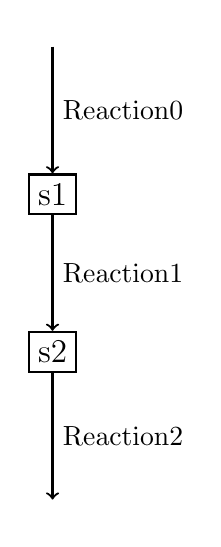
\begin{tikzpicture}[node distance=2cm]

	\node [text=black](IN) {};
	\node [species, below of = IN] (A) {\large s1};
	\node [species, below of = A] (B) {\large s2};
	\node [below of = B] (C) {};

	\draw [->, reactionLineStyle] (IN) to node[right, black] {Reaction0} (A);
	\draw [->, reactionLineStyle] (A) to node[right, black] {Reaction1}  (B);
	\draw [->, reactionLineStyle] (B) to node[right, black] {Reaction2} (C);
\end{tikzpicture}
\end{document}
